\documentclass{article}
\usepackage{graphicx} % Required for inserting images
\usepackage{amsmath,amssymb, amsthm}
\usepackage{algorithm}
\usepackage{algorithmic}

\title{Advanced Trees Notes}
\author{Kylind Reagan}
\date{September 2025}

\begin{document}

\maketitle

\section{Red Black Trees}
\begin{figure}[htp]
    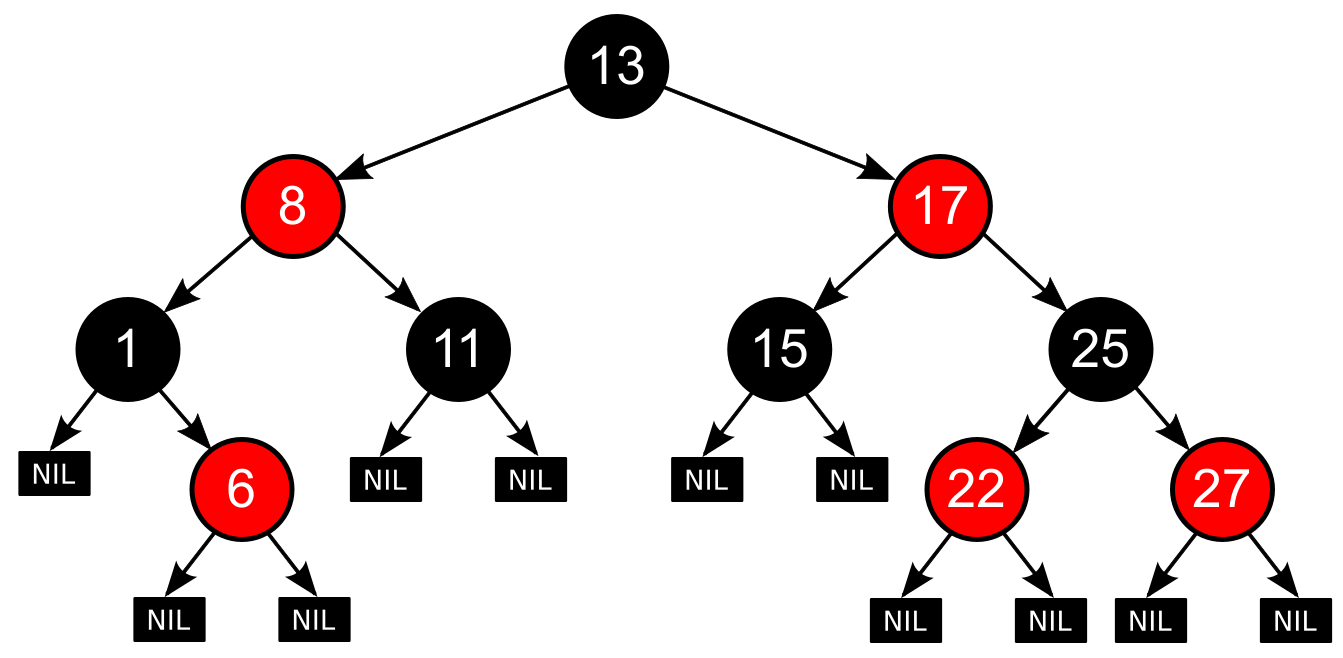
\includegraphics[width=\textwidth]{RBT.png}
    \caption{Red Black Tree Example}
    \label{tab:placeholder}
\end{figure}
\subsection{Introduction}
BST- $log(n)$ when balanced but has a worst case of $n$.\\
AVL trees balance BSTs, but balancing can be costly.\\
What if we could $\textit{approximately}$ balance a tree?\\
Give node has a color property, a $\textbf{Red Black Tree}$ has the following \\ properties...
\begin{enumerate}
    \item Every node is either red or black.
    \item Root is black.
    \item Every leaf (NIL) is black.
    \item If a node is red, both children are black.
    \item For each node, all paths from node to descendant leaves contain the same number of black nodes.
\end{enumerate}
Theorem: A red black tree w/ $n$ internal nodes has height of $\textit{at most}$ $2log(n+1)$.
\begin{proof}
We start by showing a subtree rooted at any node $x$ contains at least $2^{bh(x)}-1$ internal nodes where $bh(x)$ = black nodes from x to leaf (excluding $x$).\\
Base:\\
LHS: When $x$ is leaf x=0.\\
RHS: $2^{bh(x)}-1 = 2^0 - 1 = 0$.\\
Thus basis holds.\\
IH: Assume the subtree at some $x$ has at least $2^{bh(x)}-1$ internal nodes.
Inductive Step: Consider a node $x$ that has positive height and is an internal node w/ 2 children.\\
Each child has a black height of either $bh(x)$ or $bh(x) - 1$, depending on if it is red or black.\\
Since height of child is less than $x$ itself, we apply I.H. to conclude the child has at least $2^{bh(x)-1}-1$ internal nodes.\\
Then the subtree rooted at $x$ contains at least $2^{bh(x)-1}-1+2^{bh(x)-1}-1+1 = 2^{bh(x)}-1$ as desired.\\
Let $h$ be the height of the tree.\\
According to property 4, at least half of the nodes on any simple path from the root to the leaf, excluding the root, must be black.\\
Consequently, the black-height of the root must be at least $\frac{h}{2}$.\\
Thus,\\
\begin{align*}
    n &\geq 2^{\frac{h}{2}}-1\\
    n+1 &\geq 2^{\frac{h}{2}}\\
    log_2(n+1) &\geq \frac{h}{2}\\
    2log_2(n+1) &\geq h \text{ as desired.}
\end{align*}
\end{proof}
An immediate consequence of this proof is that the dynamic set operations search, min, max, successor and decessor are $log(n)$.\\
This also applies to Tree-insert and Tree-delete.\\
\subsection{Rotate}
Inserts and deletes may violate properties above (2, 4, 5) so we must sometimes rebalance the tree.\\
(Note leaves notated as sentinel nil[T])\\
\begin{algorithm}
\caption{Left-Rotate($T, x$)}
\begin{algorithmic}[1]
    \STATE $y \gets \text{right}[x]$
    \STATE $\text{right}[x] \gets \text{left}[y]$
    \IF{$\text{left}[y] \neq \text{nil}[T]$}
        \STATE $p[\text{left}[y]] \gets x$
    \ENDIF
    \STATE $p[y] \gets p[x]$
    \IF{$p[x] = \text{nil}[T]$}
        \STATE $\text{root}[T] \gets y$
    \ELSE
        \IF{$x = \text{left}[p[x]]$}
            \STATE $\text{left}[p[x]] \gets y$
        \ELSE
            \STATE $\text{right}[p[x]] \gets y$
        \ENDIF
    \ENDIF
\end{algorithmic}
\end{algorithm}
\\
Right-Rotate($T,x$) is symmetric.\\
Rotations keep properties intact during inserts and deletes.
\begin{figure}[htp]
    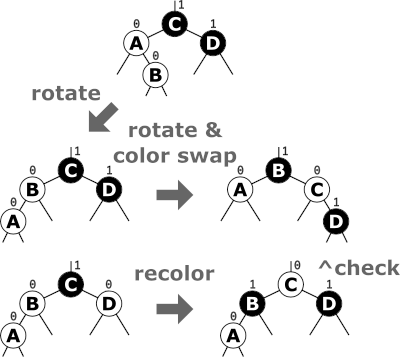
\includegraphics[width=\textwidth]{RBTinsert.png}
    \caption{Red Black Tree Rotate}
    \label{tab:placeholder}
\end{figure}
\newpage
\section{B-Trees}
\begin{figure}[htp]
    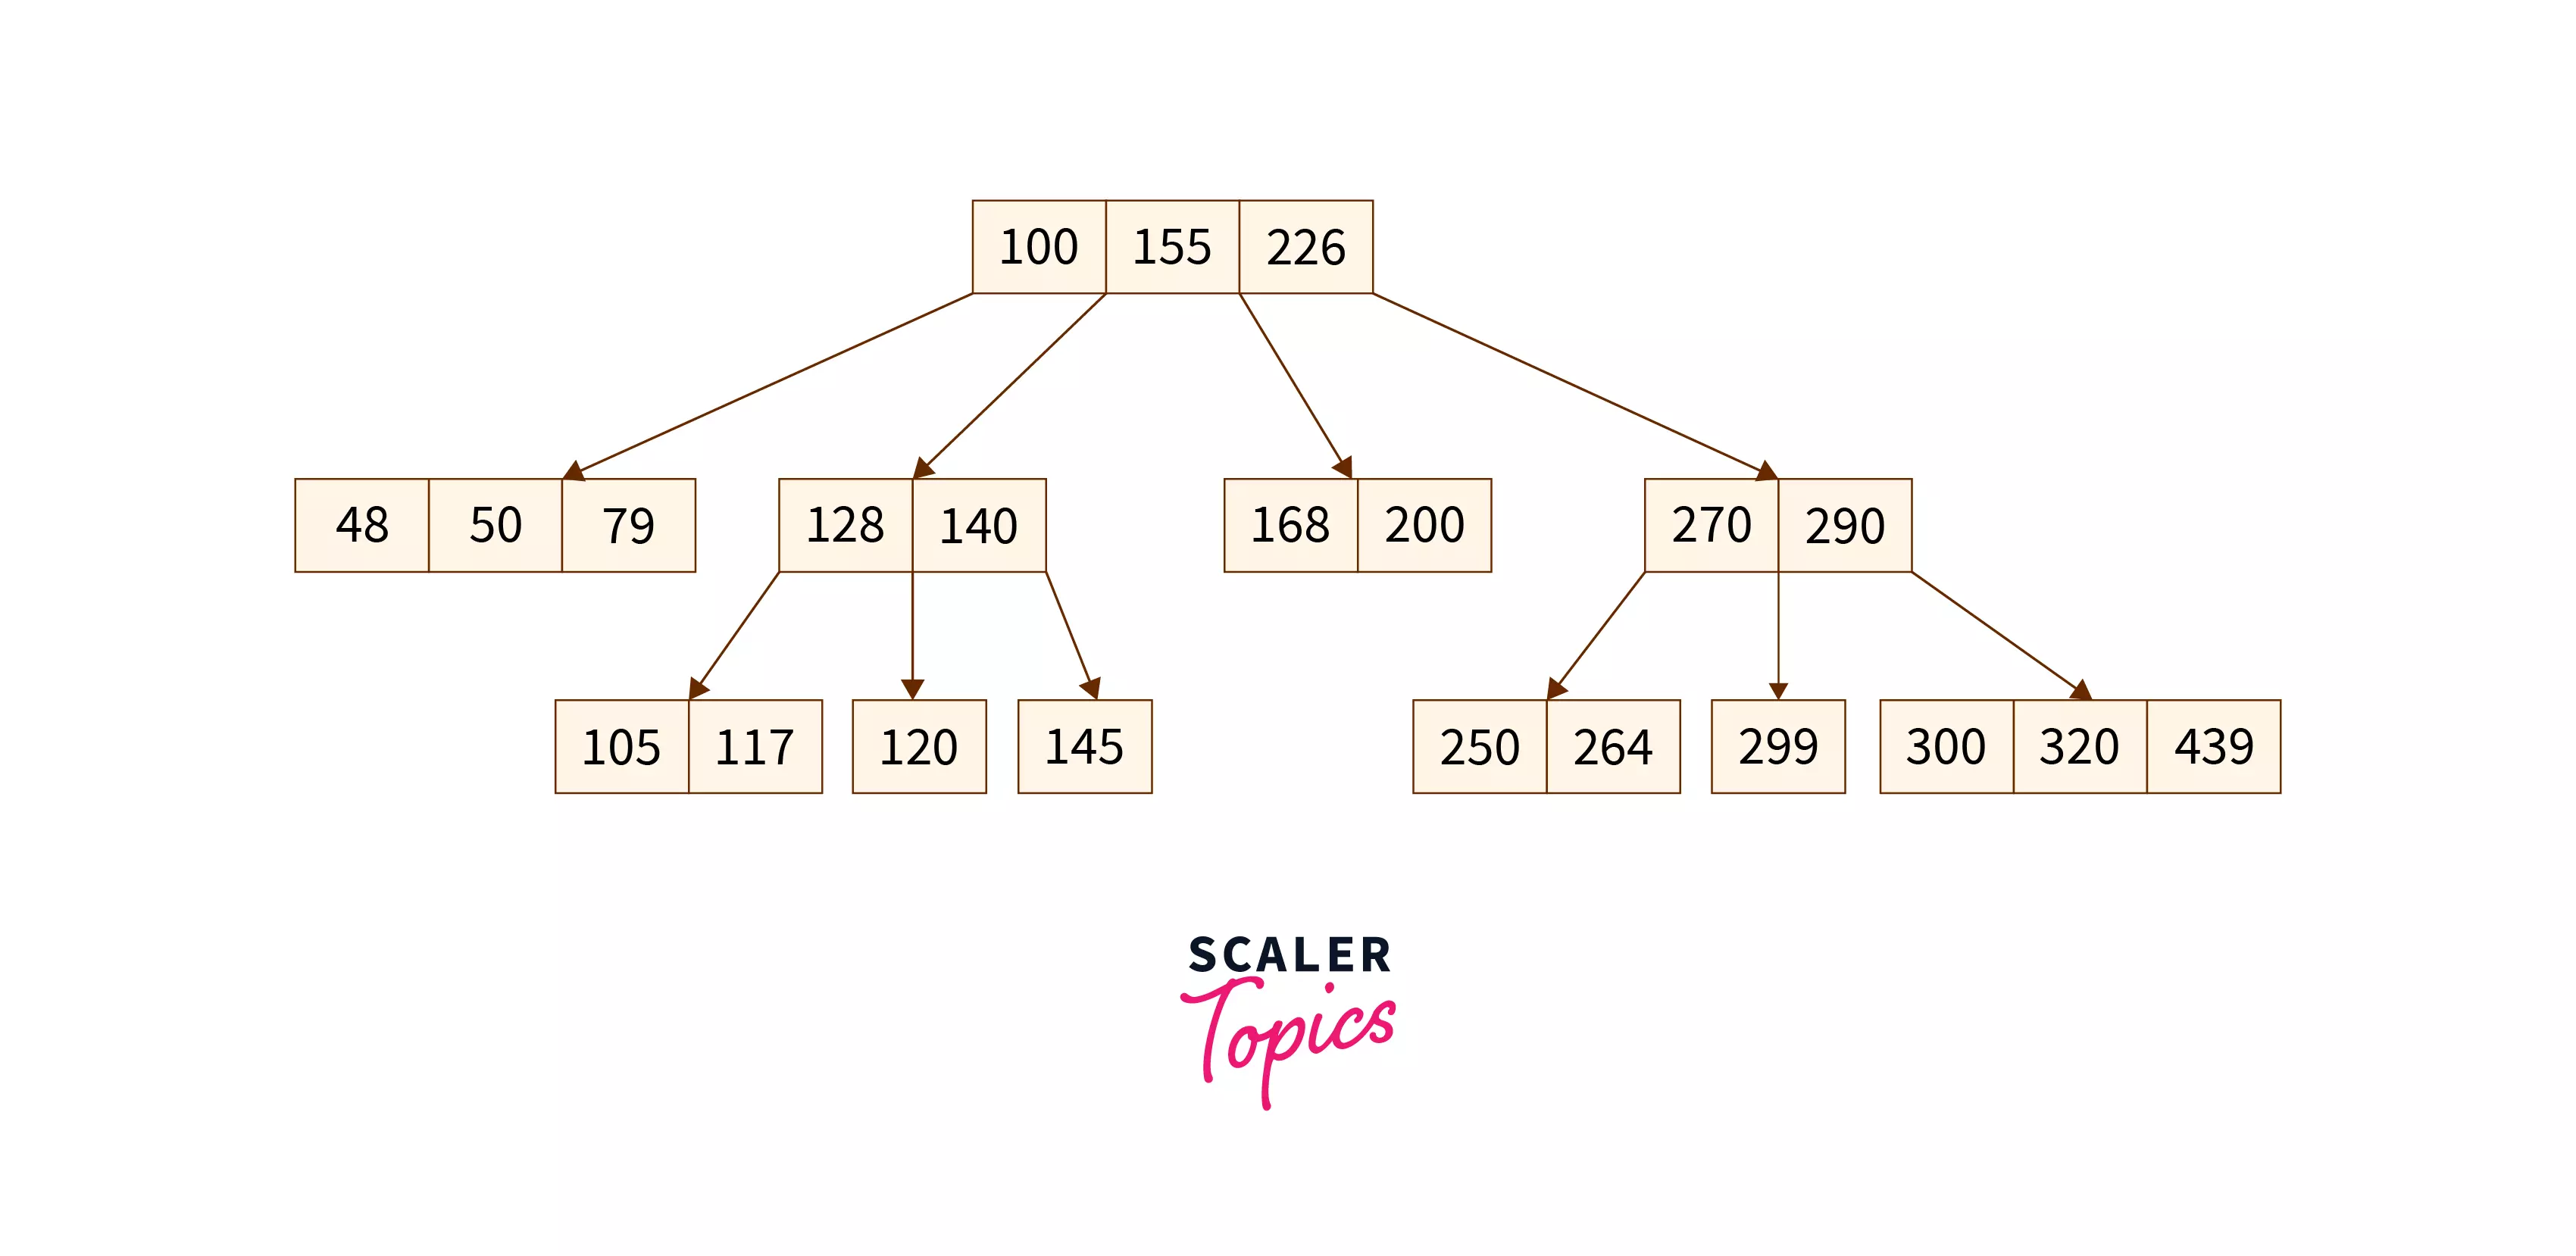
\includegraphics[width=\textwidth]{btree.png}
    \caption{B-Tree Example}
    \label{tab:placeholder}
\end{figure}
\subsection{Introduction}
$\textbf{B-trees}$ are balanced search trees designed to work well on magnetic disks or other direct secondary storage devices.\\
Similar to red black trees but optimized to lower disk I/O ops.\\
See lots of use in large databases.\\
Nodes have many children, from a handful to thousands.\\
Large "branching factor"; depends on disk.\\
Every $n$-node B-tree has height $O(log(n))$.\\
Height can be considerably less (large branching factor).\\
Can implement many dynamic set ops in $O(log(n))$.\\
If internal node $x$ has $n[x]$ keys, $x$ has $n[x]+1$ children.\\
\subsection{Memory}
Primary memory: Typically sillicon- 2 orders more expensive per bit than magnetic.\\
Secondary memory- Magnetic disk- Often exceeds amount in primary by magnitudes. Much slower as it has moving parts. Full rotation of disks = 8.33 milliseconds, could access main memory 100,000 times (100 nanoseconds).\\
Because of this, disks access several items at a time to amortize waiting.\\
A B-tree of height 2 \& 1000 keys has over a billion keys.\\
\subsection{Properties and Conventions}
A B-Tree $T$ is a rooted tree $root[T]$ w/ the following properties.\\
\begin{enumerate}
    \item Every node $x$ has the following fields:
    \begin{enumerate}
        \item $n[x] = $ number of keys in node $x$.
        \item $n[x]$ keys themselves stored in nondecreasing order so that $\text{key}_1[x] \leq \text{key}_2[x] \leq ... \leq \text{key}_{n[x]}[x]$
        \item $leaf[x] = $ a bool where $T = leaf$ \& $F =$ not $leaf$.
    \end{enumerate}
    \item Each internal node $x$ also contains $n[x] + 1$ pointers $c_1[x], c_2[x],...,c_n[x]+1$ to its children. Leaf nodes have no children so $c_i$ is undefined.
    \item The keys $key_i[x]$ separate the ranges of keys stored in each subtree: if $k_i$ is any key stored in subtree with root $c_i[x]$, then
    \begin{align*}
        k_1 \leq key_1[x] \leq k_2 \leq key_2[x] \leq ... \leq k_{n[x]}[x] \leq k_{n[x]+1}
    \end{align*}
    \item All leaves have the same depths, which is the tree's height $h$.
    \item These are lower and upper bounds on the number of keys a node can contain. These bounds can be expressed in terms of a fixed integer $t \geq 2$ called the $\textbf{\textit{minimum degree}}$ of the B-tree.
    \begin{enumerate}
        \item Every node other than the root must have at least $t-1$ keys. Every internal node other than the root thus has at least $t$ children. If the tree is nonempty, root must have at least 1 key.
        \item Every node can contain at most $2t-1$ keys. Therefore, an internal node can have at most $2t$ children. We say a node is $full$ if it contains exactly $2t-1$ keys.
    \end{enumerate}
\end{enumerate}
The simplest tree occurs when $t=2$. Each internal node has either 2, 3, or 4 children, thus we have a 2-3-4 tree.\\
$Theorem:$ If $n \geq 1$, then for any $n$-key B-Tree $T$ of height $h$ and min degree $t \geq 2$:
\begin{align}
    h \leq log_t(\frac{n+1}{2})
\end{align}
Another common B-Tree is a $\text{B}^*$-Tree which requires each internal node to be at least $\frac{2}{3}$ full (as opposed to half full which B-Tree requires).\\
Two conventions of B-Trees:
\begin{enumerate}
    \item B-Tree root is always in main memory so disk-read never required for root.
    \item  Any nodes passed on as parameters must have already had a disk-read performed on them
\end{enumerate}
"One pass"- Never have to go back up.\\
\subsection{Operations}
Searching is like BST but with $n[x] + 1$ checks instead of 2.\\
Inserting more complicated: Adding a key as a node will not produce a valid B-Tree.\\
Insert a key into existing node. If node full: split full node around the $\textbf{median}$ key into 2 nodes with $t-1$ keys each.\\
Then insert median key into parent. If parent full: split parent and propagate up the tree.\\
As with BST, can be done inside pass from root to leaf (split as you go).\\
Deleting similar, but a little more complicated.\\
Can delete from any node, not just leaf, and will require children to be rearranged. As well, node cannot be too small.\\
\begin{figure}[htp]
    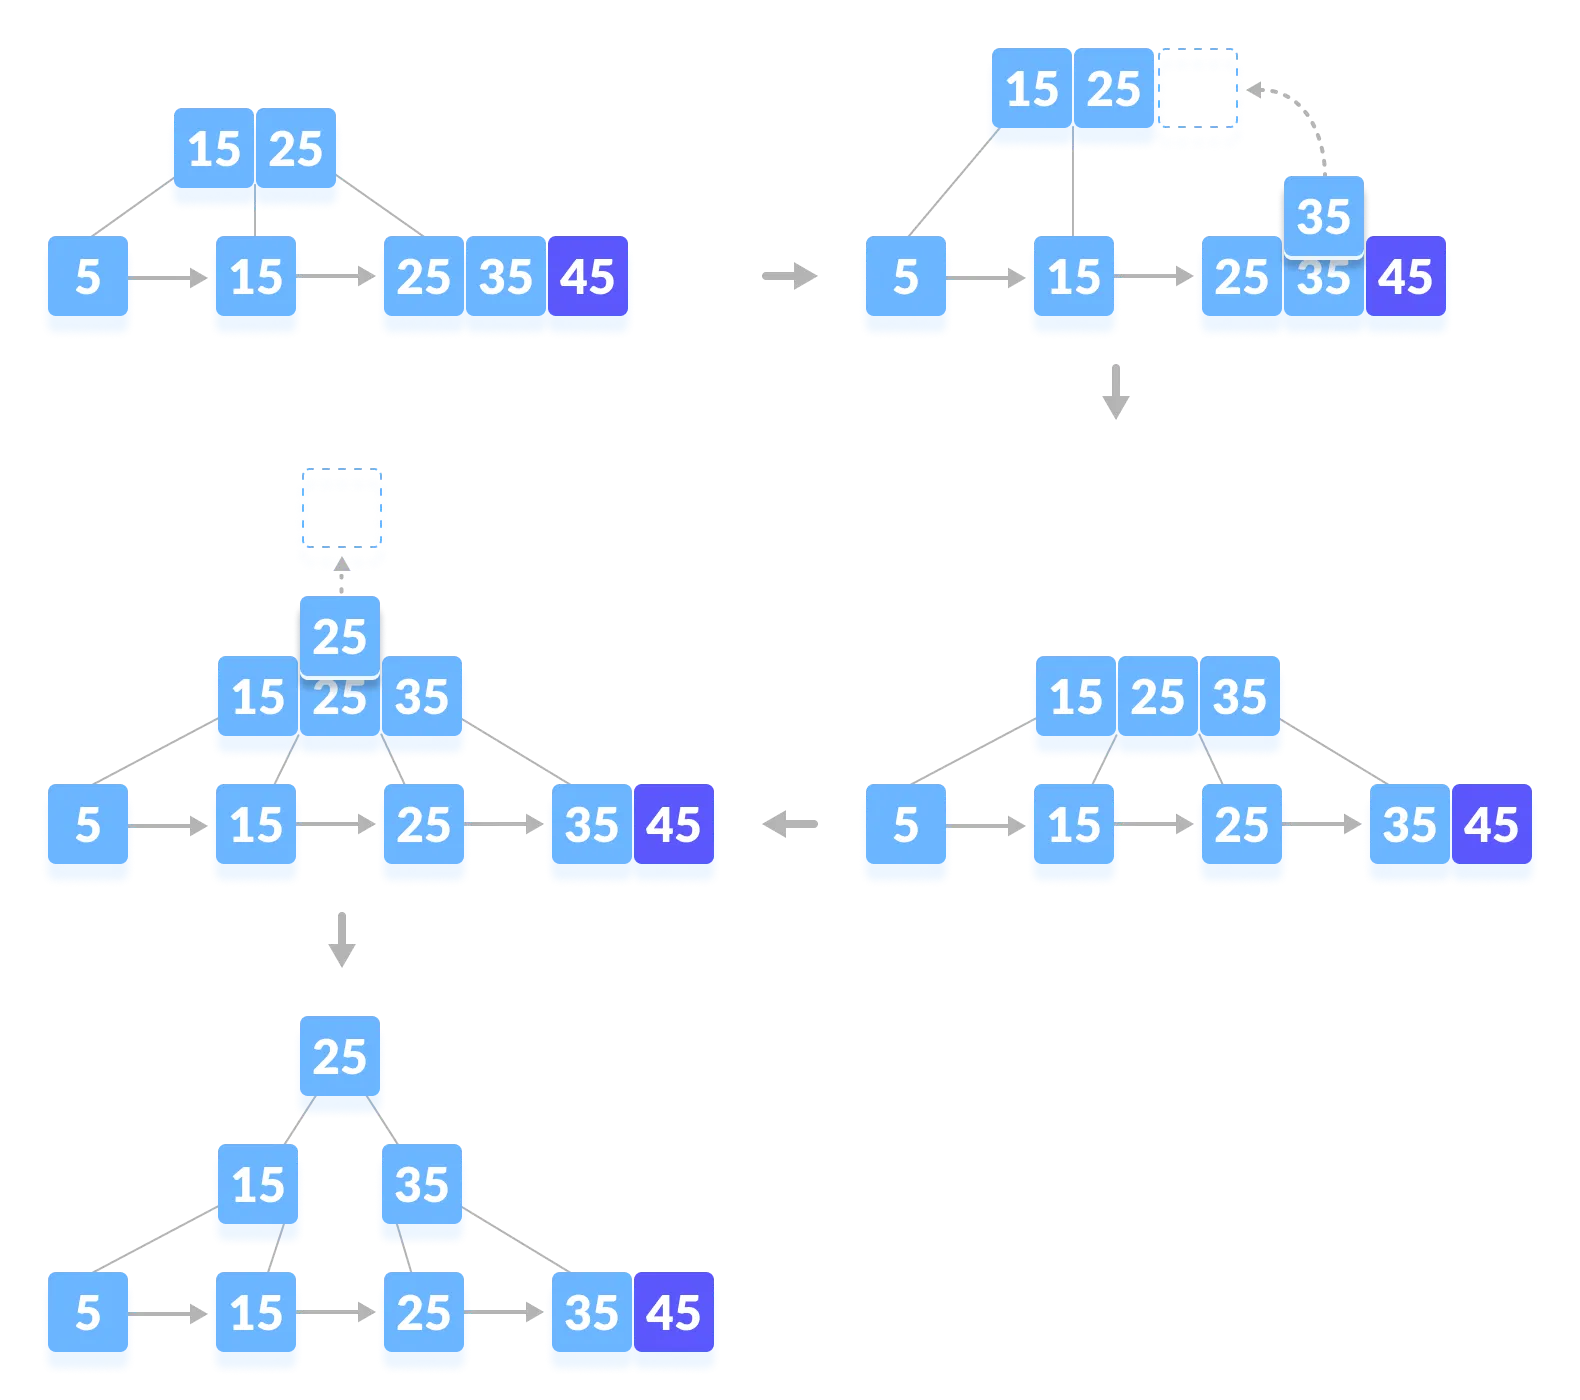
\includegraphics[width=\textwidth]{insert-5-b+tree.png}
    \caption{Insert in B-Tree}
    \label{tab:placeholder}
    
\end{figure}
\begin{figure}[htp]
    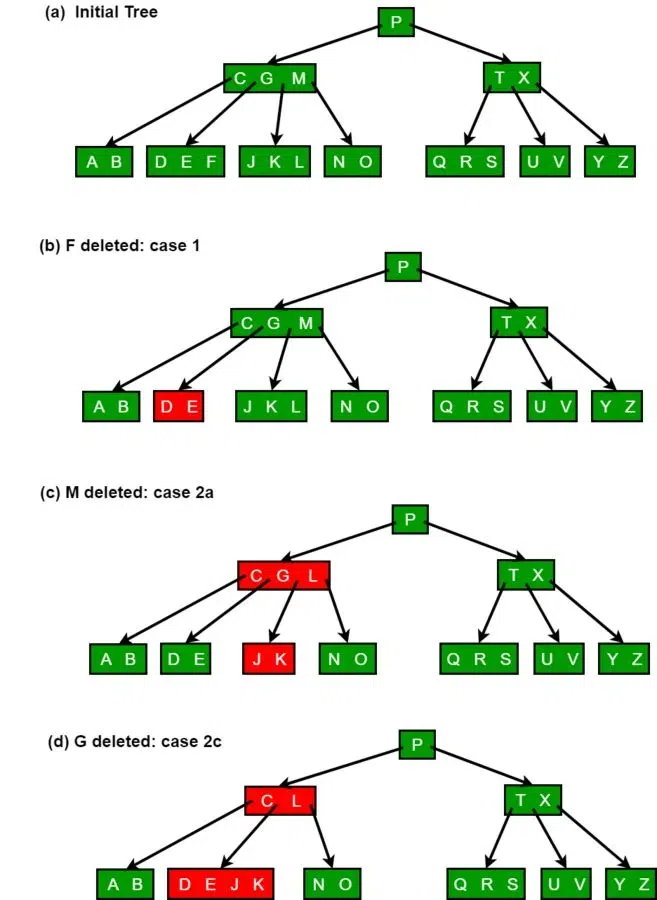
\includegraphics[width=\textwidth]{bdelete.png}
    \caption{Deletion in B-Tree}
    \label{tab:placeholder}
\end{figure}
\end{document}
